\chapter{Capa de Tecnología}
\section{Introducción}
Esta capa toma, en primer lugar, la utilización de conceptos como Nodo y Dispositivo para identificar las diferentes entidades físicas o recursos computacionales de la infraestructura del sistema \cite{BolanosCastro2019}.

Esta capa  busca establecer y conocer los diferentes elementos a nivel de software y hardware que interactúan en los procesos de negocio establecidos anteriormente, por lo tanto, es importante tener en cuenta los conceptos utilizados en la capa de negocio y en la capa de aplicación para así facilitar la identificación de los diferentes usos e interacciones que se presentan con esta capa. Para una adecuada apropiación de la conceptualización de esta capa, se implementa el uso de seis diferentes puntos de vista: infraestructura, uso de infraestructura, implementación y organización, estructura de información, realización de servicio y capas \cite{BolanosCastro2019}.

Por otra parte, es importante resaltar que, dentro de la infraestructura, un aspecto fundamental corresponde a las interacciones entre los diferentes elementos a nivel de software (componentes) y a nivel de hardware (dispositivos), que determinan la comunicación entre los conceptos de aplicación  y conceptos de negocio mencionados en las dos capas anteriores\cite{BolanosCastro2019}.

A continuación se presentan cada uno de los puntos de vista de la capa de tecnología  a partir del soporte realizado por el Área de Investigación de Análisis de datos a los investigadores de la Subdirección de Investigaciones, otras Subdirecciones y demás unidades funcionales del Instituto de Cancerología.

%-------------Punto de Vista de la Infraestructura----------%
\newpage
\section{Punto de Vista de la Infraestructura}
El Punto de Vista de la Infraestructura contiene los elementos de infraestructura de software y hardware que soportan la capa de aplicación, como dispositivos físicos, redes o software del sistema\cite{BolanosCastro2019}.

En la Figura \ref{PvInfraestructura}, se plantea el Caso para el Punto de Vista de la infraestructura con cada uno de los elementos que interactúan entre sí. 

\begin{figure}[h!]
	\centering
	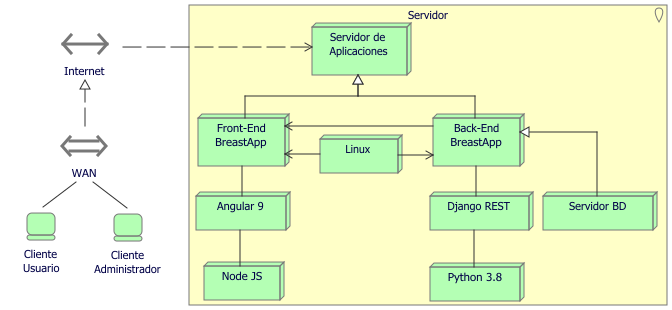
\includegraphics[width=1\linewidth]{ARQUITECTURA/imgs/CapaTecnologia/1_PvInfraestructuraTec}
	\caption{Punto de Vista de la Infraestructura}
	\label{PvInfraestructura}
\end{figure}

\begin{enumerate}[label=\textbf{\arabic*})]
	
\item  \textbf{Servidor de Aplicaciones:} Hace referencia a el nodo que se conecta directamente a la red para exponer la disponibilidad de la aplicación. Es el nodo general donde interactúan tanto componentes, como sistemas de software y demás elementos necesarios para
la aplicación.

\item \textbf{Front-End BreastApp:} Corresponde a la interfaz gráfica de usuario por la cual los investigadores y unidades funcionales del Instituto de Cancerología acceden a la aplicación, para llevar el análisis según diagnostico de cáncer de mama generado por la aplicación.

\item \textbf{Angular 9:} Hace referencia a el framework seleccionado para desarrollar  la interfaz gráfica de usuario de la aplicación BreastApp.

\item \textbf{Node JS:} Es el entorno basado en JavaScript imprescindible para poder usar el framework de Angular 9.

\item \textbf{Back-End BreastApp:} Hace referencia a el desarrollo de la lógica para la generación de la capa de servicios REST para las diferentes funcionalidades necesarias para generar el diagnostico relacionado con el cáncer de mama.

\item \textbf{Django:} Hace referencia a el framework seleccionado para desarrollar la capa de servicios REST para la aplicación BreastApp.

\item \textbf{Python 3.8:} Corresponde a el lenguaje de programación seleccionado para el desarrollo del Back-End de la aplicación BreastApp.

\item \textbf{Linux:} Este sistema de software es el sistema operativo donde se desarrolla el Back-End y Front-End de la aplicación BreastApp.

\item \textbf{Servidor BD:} Este sistema de software hace referencia a la persistencia de los datos de la aplicación BreastApp. Se realiza  automáticamente en el Back-End de la aplicación por medio del framework Django.

\item \textbf{Internet:} Hace referencia a el acceso a la aplicación  través de la red, debido a que los  investigadores y unidades funcionales del Instituto de Cancerología podrán acceder desde sus casas o lugares externos.

\item \textbf{WAN:}  Debido a  que los usuarios pueden acceder desde cualquier punto,
es necesario una red de área amplia que reúna varias redes locales y brinde la conexión a los investigadores y unidades funcionales del Instituto de Cancerología. 

\item \textbf{Cliente:} En la aplicación BreastApp, existen dos tipos de clientes:

\begin{itemize}
	\item  \textbf{\textit{Cliente Usuario:}} Hace referencia a los  investigadores y unidades funcionales del Instituto de Cancerología.
	
	\item  \textbf{\textit{Cliente Administrador:}} Hace referencia a las personas autorizadas de administrar el uso y funcionamiento de la aplicación BreastApp, así como utilizar la información del Instituto de Cancerología de manera pertinente.
\end{itemize}
\end{enumerate}

%-------------Punto de Vista de la Infraestructura----------%
\newpage
\section{Punto de Vista del Uso de la Infraestructura}
El Punto de Vista del uso de la  Infraestructura describe como las aplicaciones son compatibles con la infraestructura de software y hardware. Es muy útil para determinar los requisitos de
rendimiento y calidad de la infraestructura basados en las demandas de las diversas aplicaciones que la utilizan \cite{BolanosCastro2019}.

En la Figura \ref{PvUsoInfraestructura}, se plantea el Caso para el Punto de Vista del Uso de la infraestructura con cada uno de los elementos que interactúan entre sí. 

\begin{figure}[h!]
	\centering
	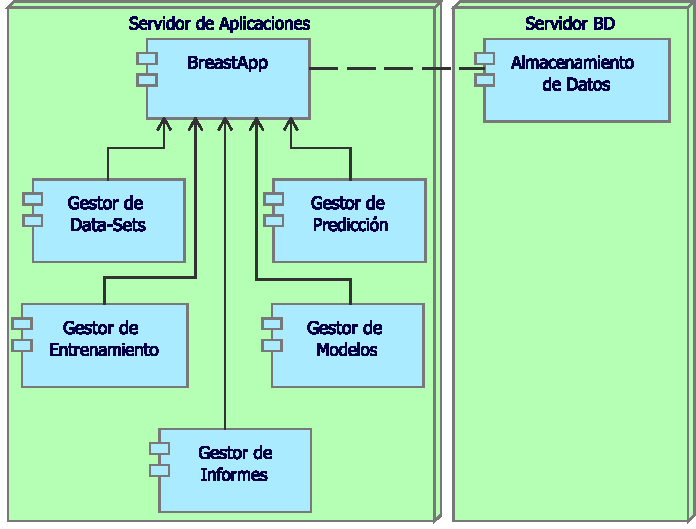
\includegraphics[width=1\linewidth]{ARQUITECTURA/imgs/CapaTecnologia/2_PvUsoInfraestructuraTec}
	\caption{Punto de Vista del Uso de la Infraestructura}
	\label{PvUsoInfraestructura}
\end{figure}


\begin{enumerate}[label=\textbf{\arabic*})]
\item  \textbf{Servidor de Aplicaciones:} En este servidor, interactúan diferentes componentes de la aplicación de BreastApp y se comunica con mas servidores a través de dichos componentes. Los componentes se describen a continuación:

\begin{itemize}
\item  \textbf{\textit{Gestor de Modelos:}} Este componente es usado por el componente principal de BreastApp.En este componente se maneja el proceso Crear modelos.
		
\item  \textbf{\textit{Gestor de Predicción:}}Este componente es usado por el componente principal de BreastApp.En este componente se maneja el proceso de diagnosticar el padecimiento de cáncer de mama.
			
\item  \textbf{\textit{Gestor de Data-Sets:}}Este componente es usado por el componente principal de BreastApp.En este componente se maneja el proceso de carga  y gestión de Data-Sets para ser almacenados en el sistema.
				
\item  \textbf{\textit{Gestor de Entrenamiento:}}Este componente es usado por el componente principal de BreastApp. En este componente se maneja el proceso de entrenamientos de los modelos de Machine Learning haciendo uso de los Data-Sets  que estén almacenados en el sistema.
					
\item  \textbf{\textit{Gestor de Informes:}}Este componente es usado por el componente principal BreastApp.En este componente se maneja el proceso de generar informes con detalles del diagnóstico.				
\end{itemize}

\item  \textbf{Servidor BD:}  Este sistema de software hace referencia a la persistencia de los datos de la aplicación BreastApp. Se realiza  automáticamente en el Back-End de la aplicación por medio del framework Django. Este servidor hace uso del componente que se describe a continuación:
\begin{itemize}
	\item  \textbf{\textit{Almacenamiento de Datos:}} Este componente hace referencia a la persistencia de la aplicación BrastApp. En este se desarrollan las funciones CRUD de la Capa de servicios REST implementada en el Back-End de la aplicación.
\end{itemize}

\end{enumerate}

%-------------Punto de Vista del Uso la Infraestructura----------%
\newpage
\section{Punto de Vista de Implementación y Organización}
El Punto de Vista de implementación y Organización describe como se despliegan una o más aplicaciones en la infraestructura. Este punto de vista comprende la asignación de aplicaciones y componentes lógicos a artefactos físicos \cite{BolanosCastro2019}.

En la Figura \ref{PvImpleOrg}, se plantea el Caso para el Punto de Vista de Implementación y Organización con cada uno de los elementos que interactúan entre sí. 

\begin{figure}[h!]
	\centering
	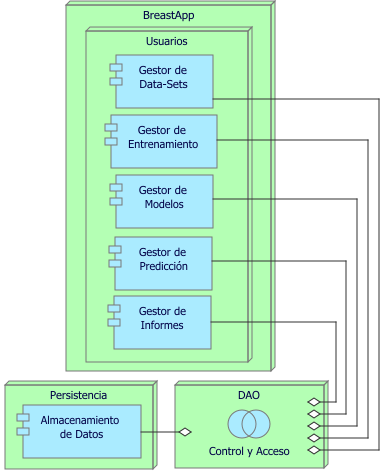
\includegraphics[width=0.65\linewidth]{ARQUITECTURA/imgs/CapaTecnologia/3_PvImplementacionOrganizacionTec}
	\caption{Punto de Vista de Implementación y Organización}
	\label{PvImpleOrg}
\end{figure}

\begin{enumerate}[label=\textbf{\arabic*})]
	
\item  \textbf{BreastApp:} Este sistema de Software representa a la aplicación en donde se desarrollan los componentes correspondientes para el diagnóstico de cáncer de mama. En este caso se tiene un nodo el cual interactúa con los componentes de este sistema.

\item  \textbf{Usuarios:} Este nodo contiene los componentes que tienen directa relación con los investigadores y unidades funcionales del Instituto de Cancerología y sus diferentes funciones. En este caso, se especifica un componente agregado a la colaboración de aplicación
\textit{Control} y \textit{Acceso}.

\begin{itemize}
\item  \textbf{\textit{Gestor de Modelos:}} En este componente se maneja el proceso de crear modelos de Machine Learning.
			
\item  \textbf{\textit{Gestor de Predicción:}} En este componente se maneja el proceso de diagnosticar el padecimiento de cáncer de mama.
				
\item  \textbf{\textit{Gestor de Data-Sets:}}En este componente se maneja el proceso de carga  y gestión de Data-Sets para ser almacenados en el sistema.
					
\item  \textbf{\textit{Gestor de Entrenamiento:}}En este componente se maneja el proceso de entrenamientos de los modelos de Machine Learning haciendo uso de los Data-Sets  que estén almacenados en el sistema.
						
\item  \textbf{\textit{Gestor de Informes:}}En este componente se maneja el proceso generar informes con detalles del diagnóstico.
\end{itemize}

\item  \textbf{Persistencia:} Este nodo hace referencia a la persistencia de la aplicación. Tiene el componente encargado de el almacenamiento y uso de información. Además, esta agregado a la colaboración de aplicación \textit{Control} y \textit{Acceso}.

\begin{itemize}
\item  \textbf{\textit{Almacenamiento de Datos:}} Este componente hace referencia a la persistencia de la aplicación BreastAPP. En este se desarrollan las funciones CRUD de la Capa de servicios REST implementada en el Back-End de la aplicación. 
\end{itemize} 

\item  \textbf{DAO:} Este sistema de software se refiere al componente que suministra la interfaz de comunicación entre la aplicación BreastApp y la base de datos. En este caso, se hace a través de una colaboración de aplicación, que se describe a continuación.

\begin{itemize}
	\item  \textbf{\textit{Control y Acceso:}} Esta colaboración trata del control de la información de las diferentes funciones de la aplicación BreastApp y su almacenamiento, y el acceso a dicha información. Tiene agregado los componentes de \textit{Gestor de Modelos},\textit{Gestor de Predicción}, \textit{Gestor de Data-Sets},\textit{Gestor de Entrenamiento}, \textit{Gestor de Informes} y \textit{Almacenamiento de Datos}.Esta colaboración es el puente para el CRUD de la Capa de servicios REST implementada en el Back-End de la aplicación BreastApp y el
	almacenamiento de los datos.
\end{itemize} 
\end{enumerate}
%-------------Punto de Vista de la Estructura de la Informacion----------%
\newpage
\section{Punto de Vista de Estructura de la Información}
El Punto de Vista de Estructura de la Información describe la estructura de la información usada en la empresa o en un proceso especifico de negocio o aplicación, en términos de tipos de datos o estructuras de clases \cite{BolanosCastro2019}.

En la Figura \ref{PvEstructuraInfo}, se plantea el Caso para el Punto de Vista de Estructura de la Información con cada uno de los elementos que interactúan entre sí. 

\begin{figure}[h!]
   \centering
   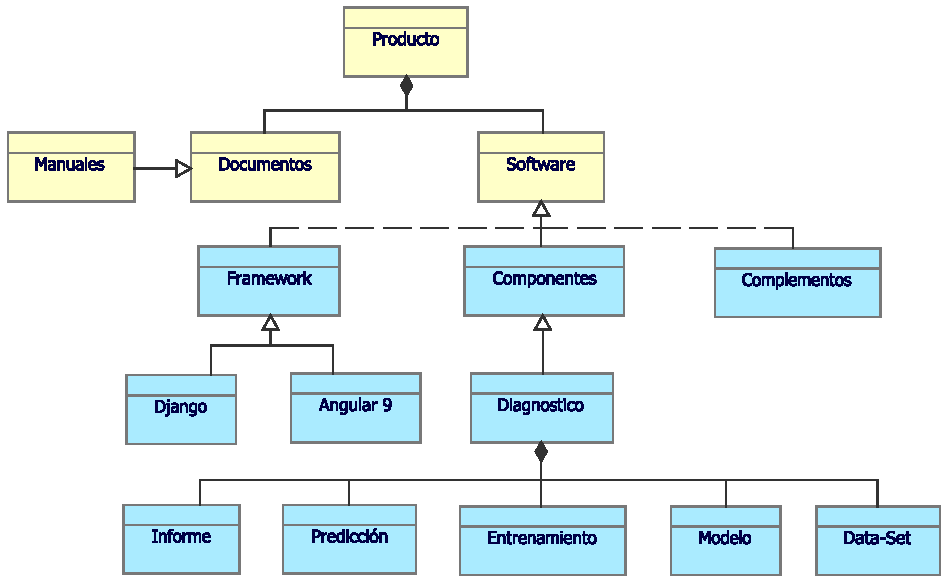
\includegraphics[width=1\linewidth]{ARQUITECTURA/imgs/CapaTecnologia/4_PvEstructuraInformacionTec}
	\caption{Punto de Vista de Estructura de Información}
	\label{PvEstructuraInfo}
\end{figure}

\begin{enumerate}[label=\textbf{\arabic*})]
	
\item  \textbf{Producto:} Este objeto de negocio se refiere al producto de software que se tiene en su totalidad. Este a su vez está compuesto por \textit{Documentos} y \textit{Software}.

\item  \textbf{Documentos:} Este objeto de negocio que hace referencia a toda la documentación correspondiente al producto como los \textit{Manuales}. Todo esto se va desarrollando gradualmente y se obtiene con el producto final.

\item  \textbf{Software:} Este objeto de negocio hace referencia a la implementación en software de la aplicación BreastApp. Este a su vez es realizado por diferentes objetos de negocio: \textit{Framework},\textit{Componentes} y \textit{Complementos}.

\item  \textbf{Framework:} En este objeto se desarrolla el software BreastApp. Esta conformado por el Framework \textit{Django} en el cual se realiza toda la lógica de la capa de servicios REST implementada en el Back-End y el Framework \textit{Angular 9} en el cual se pueden visualizar todas las funciones de la aplicación implementadas en el Front-End.

\item  \textbf{Componentes:} Este objeto contiene los diferentes componentes que interactúan en la aplicación BreastApp. Es una especialización del objeto \textit{Diagnostico} el cual es el resultado final de la aplicación y que se encuentra compuesto por los objetos \textit{Informe},\textit{Predicción},\textit{Entrenamiento},\textit{Modelo} y \textit{Data-Set}.

\item  \textbf{Complementos:} Este objeto que se refiere a los diferentes complementos utilizados en la aplicación BreastApp.En este caso se tienen complementos para la generación  de la persistencia de los datos, el diseño del Front y la publicación y consumo de la capa de servicios de la aplicación.
\end{enumerate}

%-------------Punto de Vista de Realización del Servicio----------%
\newpage
\section{Punto de Vista de Realización del Servicio}
El Punto de Vista de Realización de Servicio describe cómo uno o más servicios de negocio son realizados por un proceso fundamental o, algunas veces, por componentes de aplicación. Esto forma el puente entre productos  y las vistas de los procesos de negocio \cite{BolanosCastro2019}.

En la Figura \ref{PvRealizaServicio}, se plantea el Caso para el Punto de Vista de Realización del Servicio con cada uno de los elementos que interactúan entre sí. 

\begin{figure}[h!]
	\centering
	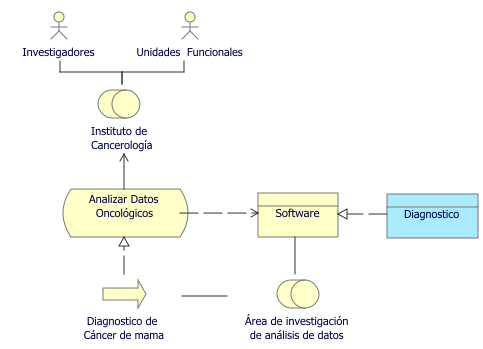
\includegraphics[width=1\linewidth]{ARQUITECTURA/imgs/CapaTecnologia/5_PvRealizacionServicioTec}
	\caption{Punto de Vista de Realización de Servicio}
	\label{PvRealizaServicio}
\end{figure}


\begin{enumerate}[label=\textbf{\arabic*})]
	
\item  \textbf{Analizar Datos Oncológicos:}  Este servicio realiza el análisis de los datos entregados por  los investigadores de la Subdirección de Investigaciones, otras Subdirecciones y demás unidades funcionales del Instituto de Cancerología para generar diagnósticos oncológicos. Es realizado por el proceso de \textit{Diagnostico de Cáncer de mama} y usado por el \textit{Instituto de Cancerología}.

\item  \textbf{Diagnostico de Cáncer de mama:}  Este proceso cumple el objetivo dar soporte a los investigadores de la Subdirección de Investigaciones, otras Subdirecciones y demás unidades funcionales del Instituto de Cancerología con respecto al análisis de datos oncológicos. Tiene asignado el rol \textit{Área de investigación de análisis de datos}.

\item  \textbf{Área de investigación de análisis de datos:}  Corresponde al área de investigación la cual da soporte a los investigadores de la Subdirección de Investigaciones, otras Subdirecciones y demás unidades funcionales del Instituto de Cancerología por medio reportes generados con base a los datos solicitados.Esta asignado al proceso \textit{Diagnostico de Cáncer de mama}.

\item  \textbf{Instituto de Cancerología :} Este rol de aplicación corresponde a los diferentes usuarios del Instituto de Cancerología. Tienes asociado el actor \textit{Investigadores} y el actor \textit{Unidades funcionales }. Estos roles se describen a continuación: 
\begin{itemize}
	\item  \textbf{\textit{Investigadores :}}  Este rol está conformado por todos los grupos de investigación en cáncer del país registrados ante Colciencias y adicionalmente, con representantes de diferentes tipos de usuarios del conocimiento generado por la investigación como son las sociedades médicas, los prestadores de servicios oncológicos, los aseguradores, las autoridades sanitarias y los pacientes entre otros. 
	
	\item  \textbf{\textit{Unidades Funcionales :}}  Este rol está conformado por las unidades clínicas ubicadas al interior del Instituto de Cancerología cuya función es evaluar la situación de salud del paciente con diagnóstico presuntivo de cáncer. 
\end{itemize}

\item  \textbf{Software:} Este objeto de negocio hace referencia a la implementación en software de la aplicación BreastApp. Es realizado por el objeto \textit{Diagnostico}.
\end{enumerate}

%-------------Punto de Vista de Capas----------------------------------%
\newpage
\section{Punto de Vista de Capas}
El Punto de Vista de capas describe varias los aspectos de una arquitectura empresarial en un diagrama como resultado del uso de la relación de agrupación para  una partición natural de todo el conjunto de objetos y relaciones que pertenecen a el modelo \cite{BolanosCastro2019}.

En la Figura \ref{PvCapas}, se plantea el Caso para el Punto de Vista de Capas con cada uno de los elementos que interactúan entre sí. 

\begin{figure}[h!]
	\centering
	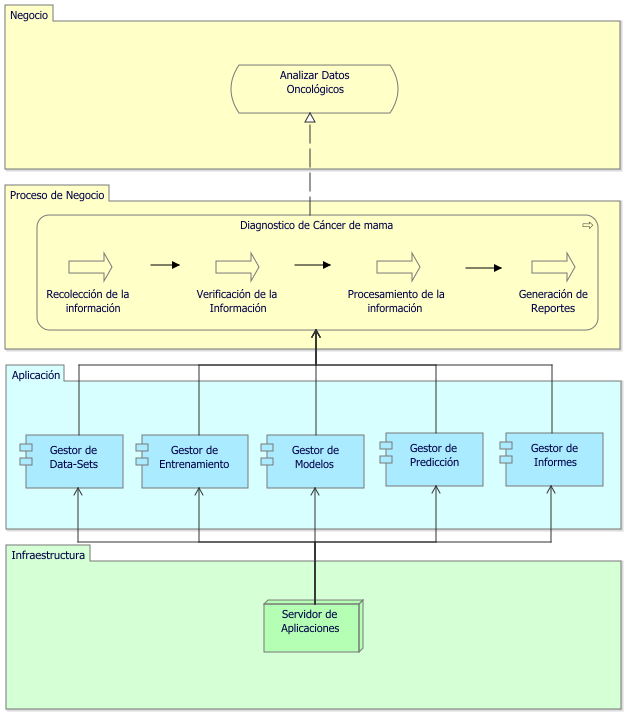
\includegraphics[width=0.8\linewidth]{ARQUITECTURA/imgs/CapaTecnologia/6_PvCapasTec}
	\caption{Punto de Vista de Capas}
	\label{PvCapas}
\end{figure}

\begin{enumerate}[label=\textbf{\arabic*})]
	
\item  \textbf{Negocio:} Esta capa expone un servicio importante el cual fue planteado con anterioridad en la Capa de Negocio. Estos  servicio es realizado por un proceso especifico, expuesto en la siguiente capa del modelo de Proceso de Negocio. La descripción de los servicios
	se expone a continuación:
	\begin{itemize}
		\item  \textbf{\textit{Analizar Datos Oncológicos:}} Este servicio realiza el análisis de los datos entregados por  los investigadores de la Subdirección de Investigaciones, otras Subdirecciones y demás unidades funcionales del Instituto de Cancerología para generar diagnósticos oncológicos.Es realizado por el proceso de \textit{Diagnostico de Cáncer de mama}.
	\end{itemize}

\item  \textbf{Proceso de Negocio:} Esta capa, expone los procesos encargados de realizar los servicios expuestos en el entorno. Son usados por distintos componentes planteados en la capa de Aplicación. La descripción de los procesos se expone a continuación.
	
	\begin{itemize}
	\item  \textbf{Diagnostico de Cáncer de mama:}  Este proceso cumple el objetivo dar soporte a los investigadores de la Subdirección de Investigaciones, otras Subdirecciones y demás unidades funcionales del Instituto de Cancerología con respecto al análisis de datos oncológicos. Esta compuesto de los siguientes procesos de negocio secuenciales: \textit{Recolección de información},\textit{Verificación de la información},\textit{Procesamiento de la información} y \textit{Generación  de Reportes}.
	\end{itemize}


\item  \textbf{Aplicación:} Esta capa, plantea los diferentes componentes que usan los procesos de negocio expuestos en la capa de Aplicación. A su vez, son usados en la capa siguiente, a través de un nodo. Esta capa esta conformada de por los siguientes componentes:

\begin{itemize}
	\item  \textbf{\textit{Gestor de Modelos:}} En este componente se maneja el proceso de crear modelos de Machine Learning.
	
	\item  \textbf{\textit{Gestor de Predicción:}} En este componente se maneja el proceso de diagnosticar el padecimiento de cáncer de mama.
	
	\item  \textbf{\textit{Gestor de Data-Sets:}} En este componente se maneja el proceso de carga  y gestión de Data-Sets para ser almacenados en el sistema.
	
	\item  \textbf{\textit{Gestor de Entrenamiento:}} En este componente se maneja el proceso de entrenamientos de los modelos de Machine Learning haciendo uso de los Data-Sets  que estén almacenados en el sistema.
	
	\item  \textbf{\textit{Gestor de Informes:}} En este componente se maneja el proceso generar informes con detalles del diagnóstico.
\end{itemize}

\item  \textbf{Infraestructura:} En esta Capa, se plantea el nodo Servidor de Aplicaciones, que usa los diferentes componentes planteados en la Capa de Aplicación. El nodo, se describe a continuación:

\begin{itemize}
\item  \textbf{Servidor de Aplicaciones:} Hace referencia a el nodo que se conecta directamente a la red para exponer la disponibilidad de la aplicación. Es el nodo general donde interactúan tanto componentes, como sistemas de software y demás elementos necesarios para la aplicación. Los componentes usados de la capa de aplicación por este nodo son: \textit{Gestor de Modelos},\textit{Gestor de Predicción}, \textit{Gestor de Data-Sets},\textit{Gestor de Entrenamiento} y \textit{Gestor de Informes}.
\end{itemize}
	
\end{enumerate}
